\documentclass[]{report}
\usepackage{listings}
\usepackage[ngerman]{babel}
\usepackage[utf8]{inputenc}
\usepackage[pdftex]{graphicx}     
\usepackage{booktabs}
\usepackage{color}
\usepackage{tabulary}

 \lstset{language=Java,
          showstringspaces=false,
          frame=single,
          numbers=left,
          basicstyle=\ttfamily\scriptsize,
          numberstyle=\tiny,
        }
% Title Page
\title{MISS \\ Mac-based Identification and Signaling Service}
\author{Fabian Schwab (fabian.schwab@uni-ulm.de)}
\begin{document}
\maketitle

%\begin{abstract}
%\end{abstract}
\chapter{Einleitung}
Um sich den Alltag zu erleichtern, werden immer mehr kleine Aufgaben auf das Smartphone bzw. Tablet ausgelagert, wodurch diese Geräte zu unseren ständigen Begleitern werden. Der auf einem Smartphone genutzte Kalender enthält alle Termine und wichtige Aufgaben, welche an bestimmten Tagen zu gewissen Zeiten zu erledigen sind. Einfache Funktionen innerhalb dieser Kalenderanwendungen erlauben es individuelle Benachrichtigungen für jeden Termin einzustellen, welche den Nutzer durch Audio, Visuelle oder Audiovisuelle Ereignisse an ein bestimmtes Ereignis erinnert.\\
Doch sind Zeitabhängige Erinnerungen nicht immer praktisch. In manchen Situationen lässt sich nicht genau festlegen wann eine Aufgabe zu erledigen ist.\\
Sollte zum Beispiel etwas bestimmtes nach der Arbeit erledigen werden, kann man dies natürlich als Zeitabhängiges Event einstellen. Verlässt man aber die Arbeit nicht zur gewohnten oder gedachten Zeit, kann diese Erinnerung zu spät erscheinen, oder wurde vom Nutzer bereits wieder vergessen, da diese schon vor Stunden erschien. \\
Hierdurch entstanden viele Anwendungen, welche auch Ortsabhängige Erinnerungen durchführen können. So lassen sich beim verlassen oder ankommen an voreingestellten Orten Erinnerungen auslösen. Zum Beispiel wäre es möglich einzustellen, dass beim verlassen der Arbeit, etwas bestimmtes erledigen sollte. \\
Damit lassen sich schon eine Vielzahl an möglichen Szenarien abdecken. Doch gibt es noch einen großen Teil, welcher weder Zeit noch Ortsgebunden bestimmt werden kann. Diese trifft vor allem auf Szenarien in Zusammenhang mit Personen zu. \\
Es lässt sich schwer vorausahnen wann und wo man eine Person antrifft womit Orts- und Zeitgesteuerte Erinnerungen entfallen. Einfache Notizen erscheinen hier noch das beste Mittel der Wahl zu sein. Doch an diese muss sich der Nutzer wieder selbst Erinnern. Dabei spielt der Zeitliche Abstand der Notiz zum erneuten treffen einer Person eine große Rolle. Je länger es her ist, desto größer ist die Wahrscheinlichkeit, dass der Nutzer nicht mehr daran denkt. \\
Bei all diesen Szenarien wäre eine personenbezogene Erinnerung von Vorteil. Doch wie ist dies am besten zu realisieren? \\ 
Die Lösung dieses Problems befindet sich bereits in der Hosentasche der meisten Menschen. Wie zu beginn erwähnt, sind Smartphones und Tablets ständig griffbereit und ein ständiger Begleiter. Da diese Geräte meist ohne Unterbrechung mit dem Internet verbunden sind, liegt die Lösung nahe, alle Aufenthaltsorte aller Nutzer auf einem zentralen Server zu speichern. Doch würde diese Lösung einige Probleme mit sich bringen. \\
Unter anderem wäre das ständige Ermitteln und Übermitteln des eigenen Standorts unerlässlich, was wiederum einen hohen Energiebedarf und einer hohen Erneuerungsrate bei schnellen Ortswechseln mit sich zieht. Auch müssten alle Nutzer die selbe Anwendung installiert haben um einen funktionsfähigen Dienst zu ermöglichen. \\
Selbst wenn diese Hürden überwindet werden würden, besteht immer noch die Gefahr, dass diese Daten missbraucht werden könnten. Die Sicherheitsmaßnahmen würden enorm sein um solch ein System gegenüber Missbrauch zu sichern. Ebenfalls müssten alle Nutzer ihr Vertrauen in dieses System setzten. Würden Nutzer ihre Internetverbindung für solch eine Anwendung absichtlich sperren oder hätten keinen Empfang, so hätte auch dieser Ansatz keinen Erfolg.\\
Ein dezentraler Ansatz, welcher keine ständige Internetverbindung benötigt und von jedem Nutzer kontrolliert werden könnte wäre somit die beste Lösung. Da keine Notwendigkeit besteht ständig wissen zu müssen wo sich eine gesuchte Person aufhält, ist eine Erinnerung nur von Interesse  wenn diese Person bzw. ihr begleitendes Smartphone sich in unmittelbarer Nähe befindet. Genau auf dieser Grundlage entstand das Projekt \textit{mac-based identification and signaling service} kurz MISS.\\
Jedes WLAN fähige Gerät muss sich beim Senden oder Empfangen von Daten und auch sonst in Gewissen abständen mit anderen WLAN Geräten in der Nähe abstimmen, ob bzw. wann die Luftschnittstelle frei zur Übertragung ist. Genau diese Kommunikation kann genutzt werden um Geräte in seiner Nähe zu erkennen und identifizieren.\\ Die einzige Information die benötigt wird, ist die MAC-Adresse des Zielgerätes. Dabei hat der Besitzer des Gerätes die volle Kontrolle, wem er diese Adresse mitteilt. \\
Der \textit{mac-based identification and signaling service} ist ein für Android geschriebener Hintergrunddienst, welcher es ermöglicht mobile oder stationäre WLAN Geräte zu erkennen. Der Service unterscheidet zwischen mobilen Geräten, die hier als \textit{Clients} bezeichnet werden und Stationen den sogenannten \textit{Stations}. Hierbei sind die \textit{Clients} Geräte die sich mit einem WLAN verbinden und \textit{Stations} die solch ein Netzwerk aufspannen. Je nach Typ werden verschiedene Informationen gesammelt und zurückgegeben. Diese Informationen werden in Kapitel \ref{lab:airodump-ng} genauer erläutert und beschrieben.\\
Sobald sich eines der gesuchten Geräte in der Nähe befindet und erkannt wird, kann eine Benachrichtigung über dessen Fund ausgelöst werden.
\chapter{Grundlagen}
Um die Funktionsweise des Service genauer verstehen zu können, sollten zunächst einige Grundlagen erklärt werden. In diesem Abschnitt werden die vom Service genutzten Technologien kurz beschrieben. Da dies keine vollständige Beschreibung darstellt, sollten die Technologien in ihren Grundzügen bekannt sein. 
\section{Kabellose Kommunikation}
Die Anzahl der Geräte die mithilfe von WLAN kommunizieren nehmen ständig zu. Bei einem Großteil dieser Geräte wird das \textit{WNIC}\footnote{Wireless Network Interface Controller}, manchmal trotz limitierter Ressourcen, nicht abgeschaltet. Trotz verschlüsselter Verbindungen werden definiert durch den \textit{IEEE 802.11} Standard einige Daten in Klartext übertragen. Diese Daten werden von MISS genutzt um Geräte in der Nähe zu erkennen und bekannte zu identifizieren. \\
Durch den \textit{IEEE 802.11} Standard werden auf der Sicherungsschicht des \textit{OSI-Modell} Datagramme, sogenannte \textit{Frames} definiert welche in spezielle Teile unterteilt sind. Jeder \textit{Frame} enthält ein \textit{MAC-Header} Feld, in dem die Absender MAC-Adresse im Klartext dargestellt ist. Durch belauschen der umliegenden Kommunikation kann so nach einer bestimmten MAC-Adresse gesucht werden. \\
Aber nicht nur Geräte die im Moment Daten austauschen können erkannt werden, sonder auch Geräte die inaktiv sind. Jedes WLAN fähige Gerät senden abhängig von der Implementierung des \textit{WNIC} Treibers periodische Pakete aus. Diese Pakete gehören zu der Gruppe der \textit{Managementframes}. \\
Bei den \textit{probe request frames} handelt es sich um Pakete, die von \textit{Clients} gesendet werden, um Informationen über naheliegende Netzwerke zu sammeln. Durch die Angabe einer \textit{SSID}\footnote{Service Set Identifier} kann im Kommunikationsbereich des Gerätes nach bestimmten Netzwerken gesucht werden. Aber auch durch Angabe der \textit{broadcast SSID} kann nach allen Netzwerken gesucht werden, die dieses Paket empfangen und darauf Antworten. Diese Pakete werden versendet egal ob das Gerät bereits mit einem Netzwerk verbunden ist oder nicht.\\
\textit{Stations} senden sogenannte \textit{beacon frames} aus. Damit geben sie periodisch ihre Präsenz, \textit{SSID} und andere Parameter bekannt. \\
Im Standard Betriebsmodus eines \textit{WNIC} ist es nicht vorgesehen, dass Pakete, die an andere MAC-Adressen gerichtet sind an höhere Schichten, bezogen auf das \textit{OSI-Modell}, weitergeleitet werden. Diese Pakete werden bereits auf der zweiten Schicht dem \textit{Data Link Layer} im \textit{WNIC} verworfen. Damit aber auch diese Pakete weitergeleitet werden, ist es notwendig den Betriebsmodus des \textit{WNIC} auf den sogenannten \textit{Monitor Mode} zu setzten. Dieser Modus wird über den Treiber des \textit{WNIC} eingestellt um muss dort aber auch implementiert sein. 
\subsection{Airodump-ng}\label{lab:airodump-ng}
\textit{Airodump-ng}\footnote{http://www.aircrack-ng.org/doku.php?id=airodump-ng} ist ein Kommandozeilenprogramm welches für das erfassen von \textit{IEEE 802.11 frames} genutzt wird und Bestandteil der \textit{Aircrack-ng suit}\footnote{http://www.aircrack-ng.org}. Mit diesem Programm lassen sich Log-Dateien erstellen, welche Informationen über alle erfassten \textit{Stations} und \textit{Clients} enthalten. Eine Auszug von solch einer Log-Datei ist in Abbildung \ref{fig:log_file} zusehen. Die nachfolgenden Auflistungen beschreiben stichpunktartig die erfassbaren Daten für \textit{Stations} und \textit{Clients}.\\ \\
\begin{figure}
    \centering
    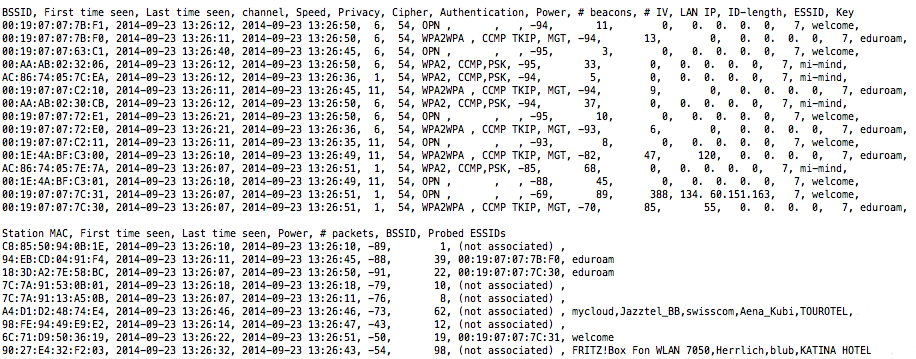
\includegraphics[width=5.0in]{bilder/log.png}
    \caption{Mit airodump-ng erstellte Log-Datei}
    \label{fig:log_file}
\end{figure}
\begin{center}
  \begin{tabulary}{\textwidth}{l | L}
\toprule
Erfassbare \textit{Station} Daten & Beschreibung \\
\midrule
BSSID & MAC-Adresse der \textit{Station} \\
First time seen & Datum und Uhrzeit der ersten Kontakts \\
Last time seen & Datum und Uhrzeit des letzten Kontakts \\
channel &  Kanal auf der die \textit{Station} sendet \\
Speed & Übertragungsgeschwindigkeit in MBit/s\\
Privacy & Privatsphäreneinstellungen \\
Cipher & Art der Verschlüsselung \\
Authentication & Genutztes Authentifizierungsprotokoll \\
Power & Signalstärke \\ 
\# beacons & Anzahl der Empfangenen \textit{beacon frames}\\
\# IV & Anzahl der Erkannten Initialisierungsvektoren \\
LAN IP &  IP Adresse \\
ID-length & Länge der ESSID \\
ESSID & Netzwerkname \\
Key & Netzwerkschlüssel falls bekannt (genutzt mit aircrack-ng) \\
\bottomrule
\end{tabulary}
\end{center} 
\begin{center}
  \begin{tabulary}{\textwidth}{l | L}
\toprule
Erfassbare \textit{Client} Daten & Beschreibung \\
\midrule
Station MAC & MAC-Adresse \textit{Clients} \\
First time seen & Datum und Uhrzeit der ersten Kontakts \\
Last time seen & Datum und Uhrzeit der letzten Kontakts \\
Power & Signalstärke \\
\# packets & Anzahl der Empfangenen \textit{frames} \\
BSSID & BSSID mit dem der \textit{Client} verbunden ist \\
Probed ESSIDs & ESSID die der \textit{Client} sucht \\
\bottomrule
\end{tabulary}
\end{center}
\section{Android}
Bevor der eigentliche Hintergrunddienst installiert werden kann, müssen einige Vorbereitungen getroffen werden. Da Google in seinem offenen Betriebssystem Android keine Möglichkeit bietet einen \textit{Monitor Mode} zu aktivieren, implementieren die Hersteller in ihren Gerätetreibern diesen auch nicht.\\
Aktuell gibt es kein Android Gerät, welches einen \textit{WNIC} besitzt, für den es einem vom Hersteller implementierten \textit{Monitor Mode} gibt. Für bestimmte Chipsätze des Herstellers Broadcom gibt es eine kleine Gruppe von Programmierer, die für die Chipsätze \textit{BCM4330} und \textit{BCM4329} eine neue Firmware geschrieben haben um eben diesen Modus zu aktivieren. Momentan werden folgende Geräte mit diesem Chipsatz unterstützt:
\begin{itemize}
\item Samsung Galaxy GS1 mit Cyanogen 7
\item Samsung Galaxy GS2 mit Cyanogen 9 oder Cynaogen 10
\item HTC Nexus One mit Cyanogen 7
\item Asus Nexus 7 mit Cyanogen 7
\end{itemize}
\subsection{Cyanogen}
Alle zuvor aufgelisteten Geräte nutzen Cyanogen\footnote{http://www.cyanogenmod.org}. Cyanogen ist eine erweiterte \textit{open source} Firmware Distribution für Smartphones und Tablets, welche auf den Android Betriebssystem basiert. Cyanogen bietet Eigenschaften und Erweiterungen die es in der offiziellen oder in der von Herstellern mit ausgelieferten Firmware nicht gibt. \\
Um Cyanogen auf einem unterstützten Gerät zu installieren, muss es zuvor \textit{gerootet} werden. Diese bedeutet, das man alle Rechte erlangt was normalerweise auch aus Sicherheitsgründen nicht vorgesehen ist. 
\subsection{bcmon.apk}
Nachdem das Gerät \textit{gerootet} wurde und Cyanogen installiert ist. Wird ein zusätzliches Programm installiert, mit dessen Hilfe der \textit{Monitor Mode} aktiviert werden kann. Das Programm \textit{bcmon} enthält dabei eine neuen Treiber für den \textit{WNIC} indem der \textit{Monitor Mode} und weitere Modi implementiert sind. Anschließend ist das Gerät für die Verwendung des MISS Hintergrunddienstes vorbeireitet. 
\chapter{Architektur und Implementierung}
In diesem Kapitel wird zunächst die grundlegende Architektur des verwendeten Dienstes erläutert und anschließend auf die Implementierung eingegangen. Dieses und nachfolgende Kapitel setzten voraus, dass Grundlagen der Programmierung in Java und Android bekannt sind. Sind diese nicht vorhanden, wird an dieser Stelle auf die Android-Entwicklerseite\footnote{http://developer.android.com} verwiesen. 
\section{Architektur}
Dieser und darauffolgende Abschnitte erklären die Funktionsweise des Service, so wie er auch implementiert wurde. Daher ist auch die Dokumentation des Quelltextes des Services hilfreich und es wird empfohlen auch dies ergänzend hierzu zu lesen. 
\subsection{Android Bound Service}
Ein Service ist eine im Hintergrund laufende Komponente welche keine direkte Interaktion mit einem Nutzer besitzt. Da ein Service kein Benutzeroberfläche benötigt, ist dieser auch nicht an den Lebenszyklus einer \textit{activity} gebunden. Im Allgemeinen werden Services genutzt um wiederkehrende und potentiell lange andauernde Aufgaben zu erledigen, wie Beispielsweise das herunterladen von Inhalten aus dem Internet oder das aktualisieren von Daten. Ebenfalls werden Services mit einer höheren Priorität ausgeführt, als Anwendungen die sich im Hintergrund befinden. Ebenfalls ist es unwahrscheinlicher, dass sie vom Betriebssystem abgeschaltet werden. \\
Zusätzlich können Services unter Android so Konfiguriert werden, dass sie neu gestartet werden sollte das Betriebssystem sie beenden. \\
Da der in diesem Projekt genutzte Service nicht immer aktiv sein soll, wird hier auf eine besondere Art eines Service zurückgegriffen. Bei dieser Art von Hintergrunddienst handelt es sich um einen in \textit{Bound Service} welcher von der selben Klasse wie ein normaler \textit{Service} ist. \\
Man kann einen \textit{Bound Service} als Server einer Client-Server-Schnittstelle betrachten. Dies ermöglicht den Android Komponenten sich an einen Service zu binden und so Anfragen zu senden und Antworten zu erhalten. Ebenso kann durch dies eine \textit{Interprocess Communication (IPC)} realisiert werden, was bei normalen Services nur mit erhöhtem Aufwand oder mit der \textit{Android Interface Definition Language (AIDL)} möglich wäre. \\
Um zwischen einem herkömmlichen und einem \textit{Bound Service} zu unterscheiden, müssen nur verschiedene Methoden implementiert werden. Der Lebenszyklus eines \textit{Bound Service} ist in Abbildung \ref{fig:lifetime} abgebildet. \\
Hierbei wird ersichtlich, dass diese Art von Service nicht immer im Hintergrund aktiv ist. Nur wenn ein Client an den Service gebunden ist wird, ist dieser aktiv. Im Gegensatz zu einem herkömmlichen Service, bei dem ein Aufruf von \textit{stopService()} genügt um diesen zu beenden, wird ein \textit{Bound Service} erst beendet, wenn sich alle Clients entbunden haben.
\begin{figure}
    \centering 
    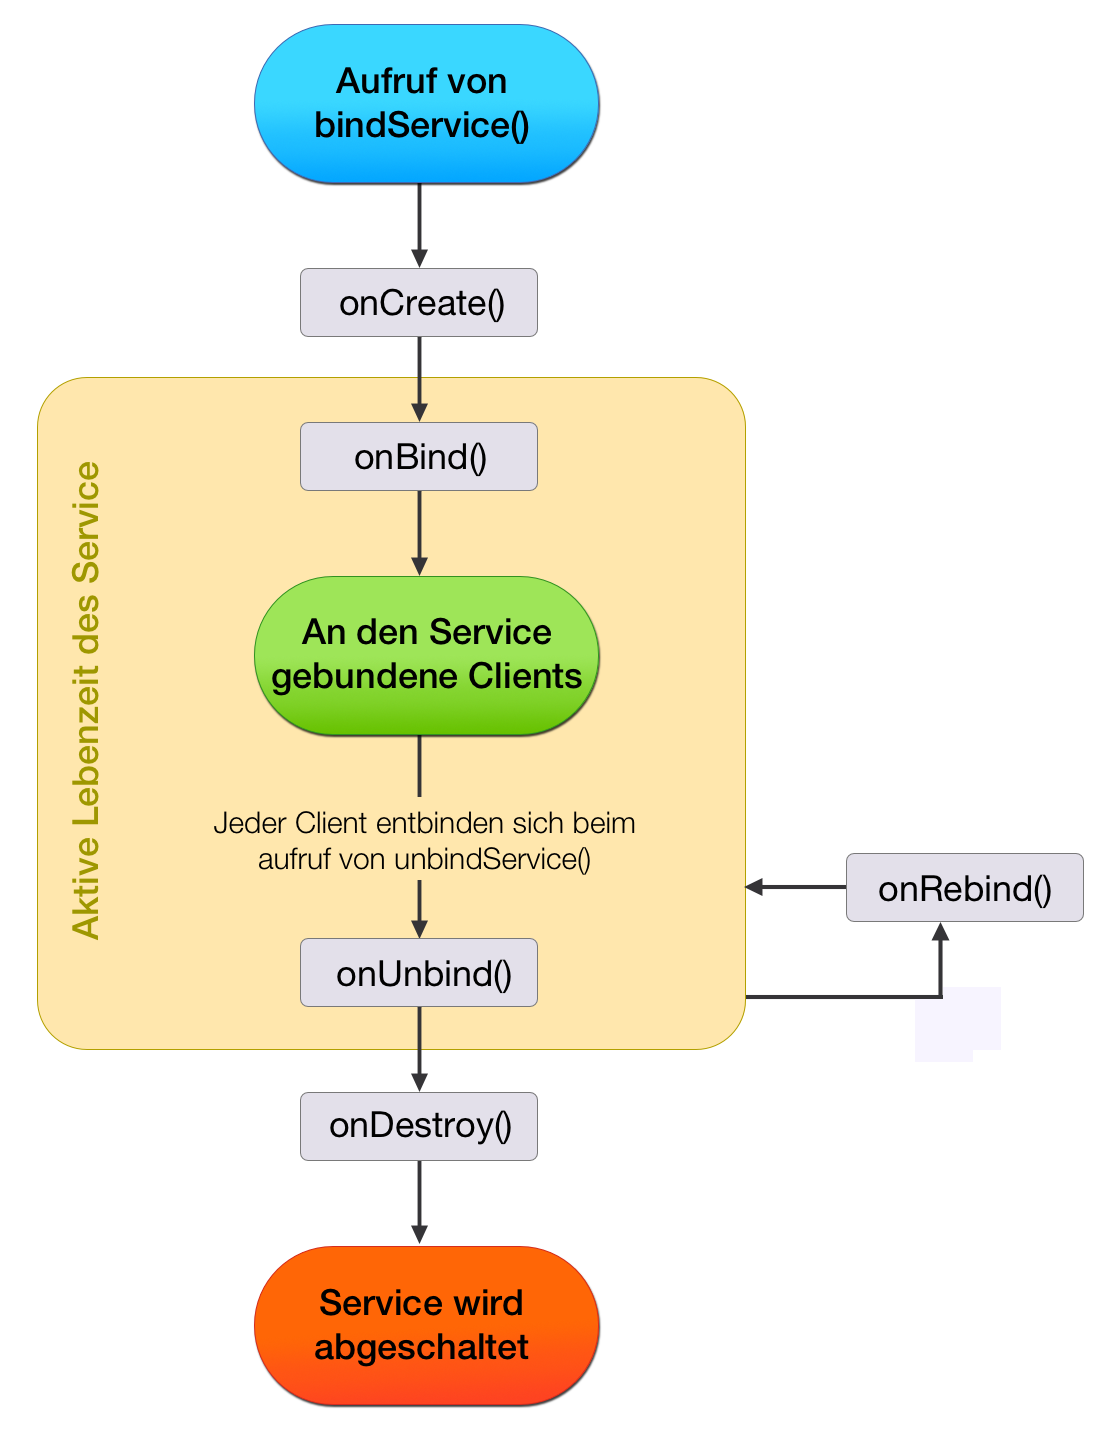
\includegraphics[width=3.0in]{bilder/boundservice.png}
    \caption{Lebenszyklus eines \textit{Bound Service}}
    \label{fig:lifetime}
\end{figure}
\subsection{Service Logik}
Der Aufbau des Service, wie er Implementiert wurde ist in Abbildung \ref{fig:uml} ersichtlich. Bindet sich eine Anwendung den Service wird dieser gestartet, sofern dieser noch nicht aktiv war. Der Service läuft als eigenständiger Prozess und verfügt über einen zusätzlichen Thread, welcher die eigentliche Arbeit übernimmt. Dies ermöglicht ein sofortiges abarbeiten ankommender Anfragen im Hauptprozess von bereits gebundenen Anwendungen oder Anwendungen die sich gerade an den Service binden möchten. \\
Aus Effizienzgründen wird der Arbeiter-Thread nur gestartet wenn Geräte gesucht werden. Zu suchenden Geräte werden an über Nachrichten den Service übermittelt, der daraufhin den Thread nach bedarf startet oder stoppt. \\
Die Aufgabe des Threads ist es alle Geräte in der Nähe zu erfassen. Dabei werden alle zu erfassenden Daten, wie in Abschnitt \ref{lab:airodump-ng} gezeigt, erfasst. Anschließend werden die gefunden Geräte mit den gesuchten Verglichen. Befindet sich ein gesuchtes unter den gefunden so benachrichtigt der Arbeiter-Thread seinen Service. Der Service sendet eine Nachricht an die entsprechende Anwendung und informiert sie über den Fund des angefragten Gerätes. \\ 
Je nach Implementierung der Zielanwendung entscheidet diese über das weitere vorgehen. In der Regel wird davon ausgegangen, das die Anwendung das gesuchte Gerät nicht mehr benötigt und dies per Nachricht an den Service übermittelt.  
Durch eine Nachricht an den Service wird das zuvor gescuhte Gerät entfernt.\\
Der Service überprüft bei jedem Empfang einer Nachricht ob der Arbeiter-Thread gestartet werden muss oder nicht. Werden Clients oder Stations gesucht wird der Thread gestartet. Sind keine Geräte mehr vorhanden wird der Thread beendet. Antwortet eine Anwendung auf den Fund eines seiner Gesuchten Geräte nicht, wird davon ausgegangen das die Anwendung unerwartet beendet wurde. Der Service entfernt die Anwendung und all ihrer Geräte welche im Zusammenhang mit ihr stehen.\\
Befinden sich danach keine gesuchten Geräte mehr im Dienst, beendet dieser den Arbeiter-Thread um Ressourcen an das Betriebssystem freizugeben. Haben sich alle Anwendungen ordnungsgemäß vom Service abgemeldet oder wurden durch eine ausbleibende Antwort entfernt, beendet sich der Service selbst da er nicht mehr benötigt wird.
\newpage
\begin{figure}[h!]
    \centering 
    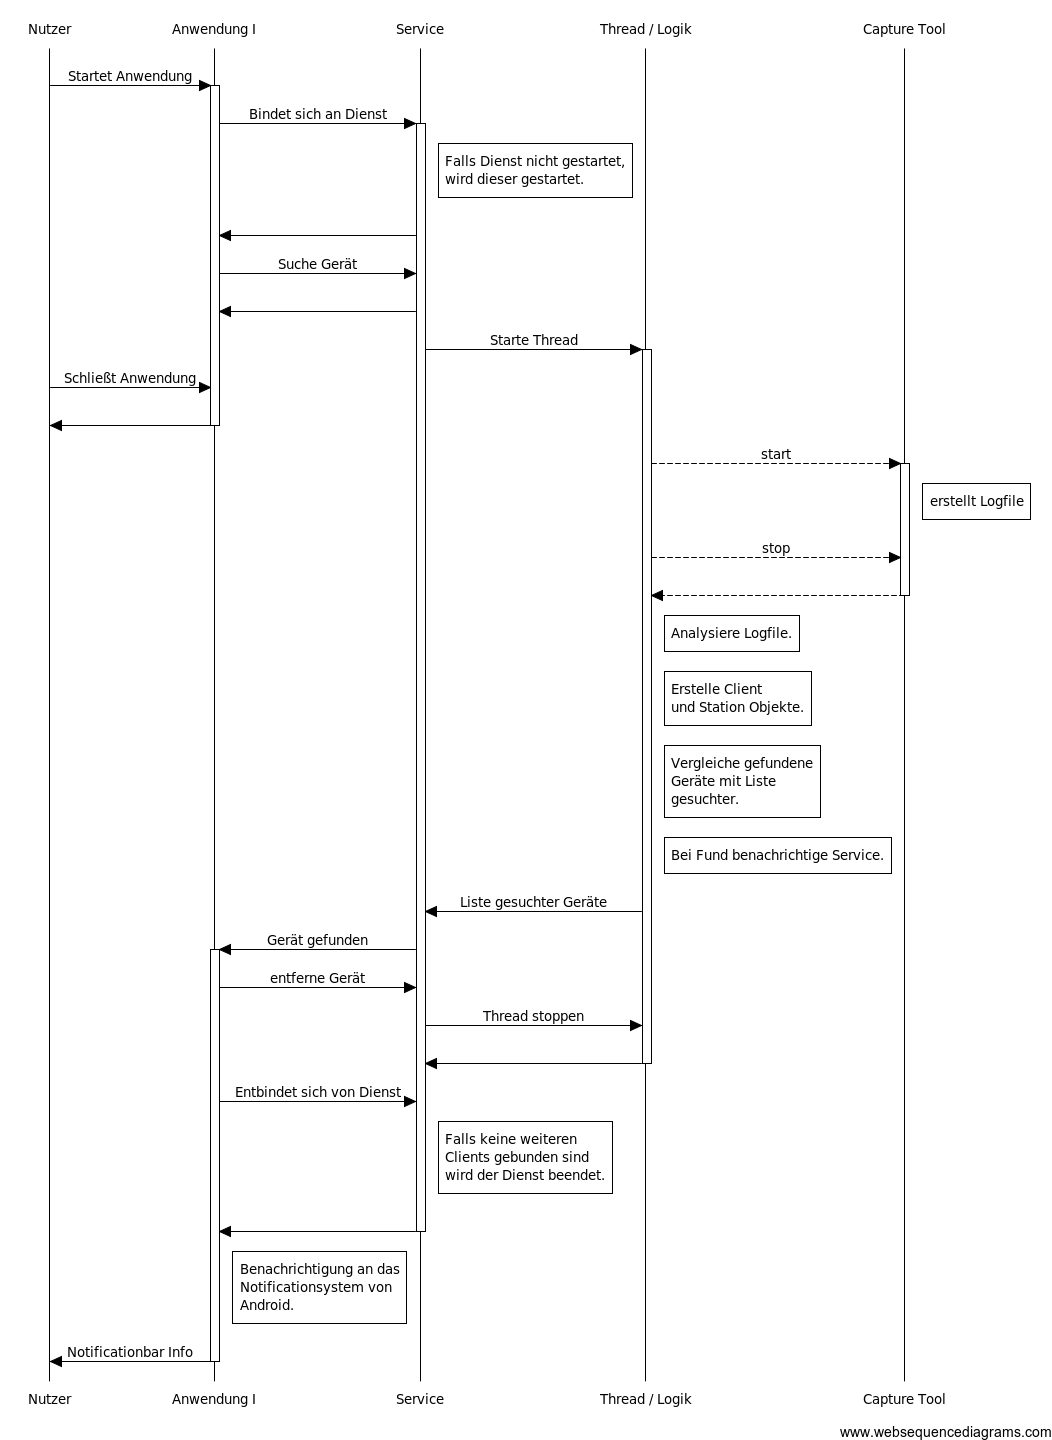
\includegraphics[width=5.0in]{bilder/uml.png}
    \caption{Anwendungsfall und Lebenszyklus des MISS als UML-Sequenzdiagramm.}
    \label{fig:uml}
\end{figure}
\section{Implementierung}
Für die Implementierung der voran gezeigten Architektur wurde das Eclipse ADT\footnote{http://developer.android.com/sdk/index.html} verwendet. Als Zielgerät wurde das Samsung Galaxy GS1 mit Cyanogen 7 gewählt. Hierbei war zu beachten, das bei der Programmierung nur Eigenschaften bis API Level 10 genutzt wurden. Dies liegt an der geringen Android Version 2.3.3 welche dem Cyanogen 7 Mod zu Grunde liegt. \\
Da im späteren Betrieb des Service Skripte benötigt werden, wurden diese zur besseren Kapselung und Entwicklung als \textit{.sh} Datei in \textit{assets} gespeichert. Dies hat den entscheidenden Vorteil, dass die programmatisch generiert werden können und nicht nach der Installation von Nutzer im Programmverzeichnis abgelegt werden müssen.\\ Ist die Luftschnittstelle auf einen anderen Gerät nicht unter der Standard Bezeichnung \textit{wlan0} zu finden, so kann dies bequem in den Skripts des Projekts geändert werden. \\ 
Folgende Skripts werden bei der Installation erstellt:
\begin{itemize}
\item removeCaptureFiles.sh
\item startCapture.sh
\item stopCapture.sh
\end{itemize}
Alle Skripte werden ausschließlich vom Arbeiter-Thread genutzt. Um unnötige Speicherbelegung zu vermeiden dient das \textit{removeCaptureFiles.sh} Skript, welches die anfallenden Log-Datei entfernt. \\ Das Starten und Stoppen von \textit{airodump-ng} wird durch die beiden anderen Skripte veranlasst, wobei \textit{startCapture.sh} wie in Listing \ref{lst:sh} einige Parameter enthält. Unter anderem wird hier das Ausgabeformat festgelegt und der \textit{WNIC} Name angegeben. Des weiteren werden die Umgebungsvariablen ergänzt, um gewisse Bibliotheken für \textit{airodump-ng} bereitzuhalten damit dies fehlerfrei Ausführt werden kann.
\begin{lstlisting}[caption={Airodump-ng Parameter}\label{lst:sh},captionpos=t] 
export PATH = $PATH:/data/data/com.bcmon.bcmon/files/tools
export LD_LIBRARY_PATH = 
  $LD_LIBRARY_PATH:/data/data/com.bcmon.bcmon/files/libs
export LD_PRELOAD = /data/data/com.bcmon.bcmon/files/libs/libfake_driver.so
airodump-ng -w /datadata/de.uulm.miss/files/capture 
  --output-format csv -w capture wlan0 2>&1
 \end{lstlisting}
In der nachfolgenden Auflistung werden alle Klassen und eine dazugehörige Beschreibung des Service MISS aufgeführt.\\ \\
\begin{center}
  \begin{tabulary}{\textwidth}{l | L}
  \toprule
  Klassenname & Beschreibung \\
  \midrule
  MainActivity.java & Wird nur bei der Installation geöffnet und erzeugt alle nötigen Skripte.\\
  MISService.java & Nimmt Anwendungsanfrage entgegen und erzeugt und kontrolliert den Arbeiter-Thread. \\
  ScanLogic.java & Arbeiter-Thread der mithilfe der Skripte alle Geräte findet und mit zu suchenden Vergleicht. \\
  FileParser.java & Erstellt Client und Station Objekte anhand des Logfiles. \\
  Client.java & Objekt welche alle für Clients erfassbaren Daten enthält. \\
  Station.java & Objekt welche alle für Stations erfassbaren Daten enthält. \\ 
  ScanOrder.java & Enthält die Liste von gesuchten Stations und Clients. \\
  \bottomrule
  \end{tabulary}  
\end{center}
Auf eine ausführliche Beschreibung der Funktionen und Parameter wurde an dieser Stelle verzichtet, da diese aus dem Quellcode entnommen werden kann. Um diesen Service zu Nutzen kann die beiliegende Anwendung, \textit{PAR} welche in Abschnitt \ref{lab:par} erläutert wird, genutzt werden. \\
Die Basisfunktionen die der Service nach außen hin bietet werden im nächsten Kapitel \ref{lab:usage} erklärt. 
\subsection{Nutzung des Service}\label{lab:usage}
Für die Nutzung des Service müssen folgende Punkte erfüllt sein:
\begin{itemize}
\item Ein unterstützter Chipsatz (\textit{BCM4330} bzw. \textit{BCM4329}) wurde verbaut.
\item Das Gerät ermöglicht \textit{root} zugriff.
\item Eine kompatible Cyanogen Firmware ist aufgesetzt.
\item Die \textit{bcmon} Anwendung ist installiert.
\item Der Service MISS ist installiert und \textit{root} Rechte wurden bewilligt.
\item Der \textit{Monitor Mode} wurde über \textit{bcmon} aktiviert.
\end{itemize}
Für eine Nutzung des Service MISS innerhalb einer Anwendung müssen nicht viele Änderungen an einer bestehenden Anwendung vorgenommen werden. Die Klasse welche mit dem Service letztendlich Kommuniziert soll, muss das Interface \textit{ServiceConnection} implementieren.\\
Hierbei müssen die Methoden \textit{onServiceConnected(ComponentName name, IBinder service)} und \textit{onServiceDisconnected(ComponentName name)} implementiert werden. Erstere wird aufgerufen wenn die Verbindung zu Service erfolgreich aufgebaut wurde und letztere wenn die Verbindung zum Service abbricht oder beendet wurde. \\
\subsubsection{An Service binden}
Listing \ref{lst:bind}  zeigt, wie eine Anwendung an den Service gebunden wird.\\ Das \textit{ServiceConnection} Objekt ist in diesem Fall die \textit{aktivity} welche \textit{ServiceConnetion} implementiert. Durch den Aufruf von \textit{bindService()} wird die Anwendung an den Service gebunden und die Methode \textit{onServiceConnected()} wird durchlaufen. 
\begin{lstlisting}[caption={Anwendung an Service binden.}\label{lst:bind},captionpos=t] 
 ServiceConnection mConnection = this;
 Intent mIntent = new Intent("de.uulm.miss.MISService");
 bindService(mIntent, mConnection, Context.BIND_AUTO_CREATE);
 \end{lstlisting}
 An dieser Stelle wird ein Objekt vom Typ \textit{Messenger} benötigt. Diese Objekt ermöglicht eine Umsetzung für eine nachrichtenbasierte Kommunikation über Prozesse hinweg. Somit lassen sich Nachrichten an den Service übermitteln und empfangen. Das Objekt wird wie in Listing \ref{lst:msg} initialisiert wobei sich die Anwendung gleich am Service registrieren. Dies wird mittels einer Nachricht an den Service und der entsprechenden Konstanten umgesetzt. 
\begin{lstlisting}[caption={Registrieren der Anwendung am Service}\label{lst:msg},captionpos=t] 
...
private final Messenger mMessenger = 
  new Messenger(new IncomingMessageHandler(this));
...
@Override
public void onServiceConnected(ComponentName name, IBinder service) {
  mServiceMessenger = new Messenger(service);
  try {
    Message regMessage = Message.obtain(null, MSG_REGISTER_APPLICATION);
    regMessage.replyTo = mMessenger;
    mServiceMessenger.send(regMessage);
  } catch (RemoteException e) {
 	// In diesem Fall wurde der Service unerwartet beendet,
 	// bevor etwas mit ihm gemacht werden konnte.
  }
}
\end{lstlisting}
 Die Konstanten mit denen zwischen Anwendung und Service kommuniziert werden kann sind im nachfolgenden Aufzählung aufgeführt.
\begin{itemize}
\item MSG\_REGISTER\_APPLICATION
\item MSG\_UNREGISTER\_APPLICATION
\item MSG\_ADD\_CLIENT
\item MSG\_ADD\_STATION
\item MSG\_REMOVE\_CLIENT
\item MSG\_REMOVE\_STATION
\item MSG\_FOUND\_DEVICE
 \end{itemize}
 Um auch eine Antworten verarbeiten zu können, muss wie in Listing \ref{lst:msg} Zeile 2 \& 3 ein \textit{Messenger} Objekte erstellt werden. Die Klasse \textit{IncomingHandler} erbt von\textit{Handler}, wobei die Methode \textit{handleMessage()} überschrieben werden muss, um die von Entwickler gewünschten Aktionen durchführen zu können. Eine Implementierung von \textit{Handler} könnte dann wie in Listing \ref{lst:handle} aussehen. In diesem Fall wird überprüft ob ein Gerät gefunden wurde. 
\begin{lstlisting}[caption={Behandelt Nachrichten die MISS an die Anwendung sendet.}\label{lst:handle},captionpos=t] 
private class IncomingMessageHandler extends Handler {
  MainActivity main;
  public IncomingMessageHandler(MainActivity parent) {
     main = parent;
  }
  @Override
  public void handleMessage(Message msg) {
  
  switch (msg.what) {
    case MSG_FOUND_DEVICE:
	  Bundle b = new Bundle();
	  b.putString("MAC", (String) msg.getData().get("MAC"));
	  b.putString("Name", (String) msg.getData().get("Name"));
	  
	  sendMessageToService(b, MSG_REMOVE_CLIENT);
      break;
    default:
      super.handleMessage(msg);
    }
  }
}
\end{lstlisting}
Ist dies der Fall wird eine neue Nachricht gesendet damit der Service das Gerät aus seiner Liste von suchenden entfernt.\\
Um Nachrichten zu senden wurde in Listing \ref{lst:handle} die Methode \textit{sendMessageToService} genutzt die in Listing \ref{lst:send} abgebildet ist. 
\begin{lstlisting}[caption={Sendet Nachrichten an den Service}\label{lst:send},captionpos=t] 
private void sendMessageToService(Bundle data, int action) {
  if (mServiceMessenger != null) {
    try {
      Message msg = Message.obtain(null, action);
      msg.setData(data);
      msg.replyTo = mMessenger;
      mServiceMessenger.send(msg);
    } 
    catch (RemoteException e) {
      ...
    }
  }
}
\end{lstlisting}
\section{Anwendungsprogramm PAR}\label{lab:par}
Um den Service MISS zu Nutzen und zu Testen wurde im Laufe des Projekts die Anwendung PAR geschrieben. PAR steht in diesem Fall für \textit{Person Aware Reminder}. Die Anwendung soll ein Einsatzgebiet des Service MISS aufzeigen. Hierbei können Erinnerungen an Personen gebunden werden. \\
Dabei werden die MAC-Adressen der Smartphone(s) der Besitzer im Adressbuch angegeben. Unter \textit{Instantmessenger} wird die Adresse mit dem Label \textit{MAC} abgelegt. Das Format muss aus Großbuchstaben bzw. Zahlen bestehen und die Blöcke müssen durch Doppelpunkte getrennt werden. Des weiteren Erlaubt die Anwendung auch Funktionen, wie sie eine einfache Erinnerungsanwendung bietet. Unter anderem sind Zeit- und Ortsabhänige Erinnerungen möglich und es besteht die Möglichkeit einfache Notizen zu schreiben. In der Abbildung \ref{fig:par} sind Auszüge aus der Anwendung zu sehen. 
\begin{figure}[h!]
    \centering 
    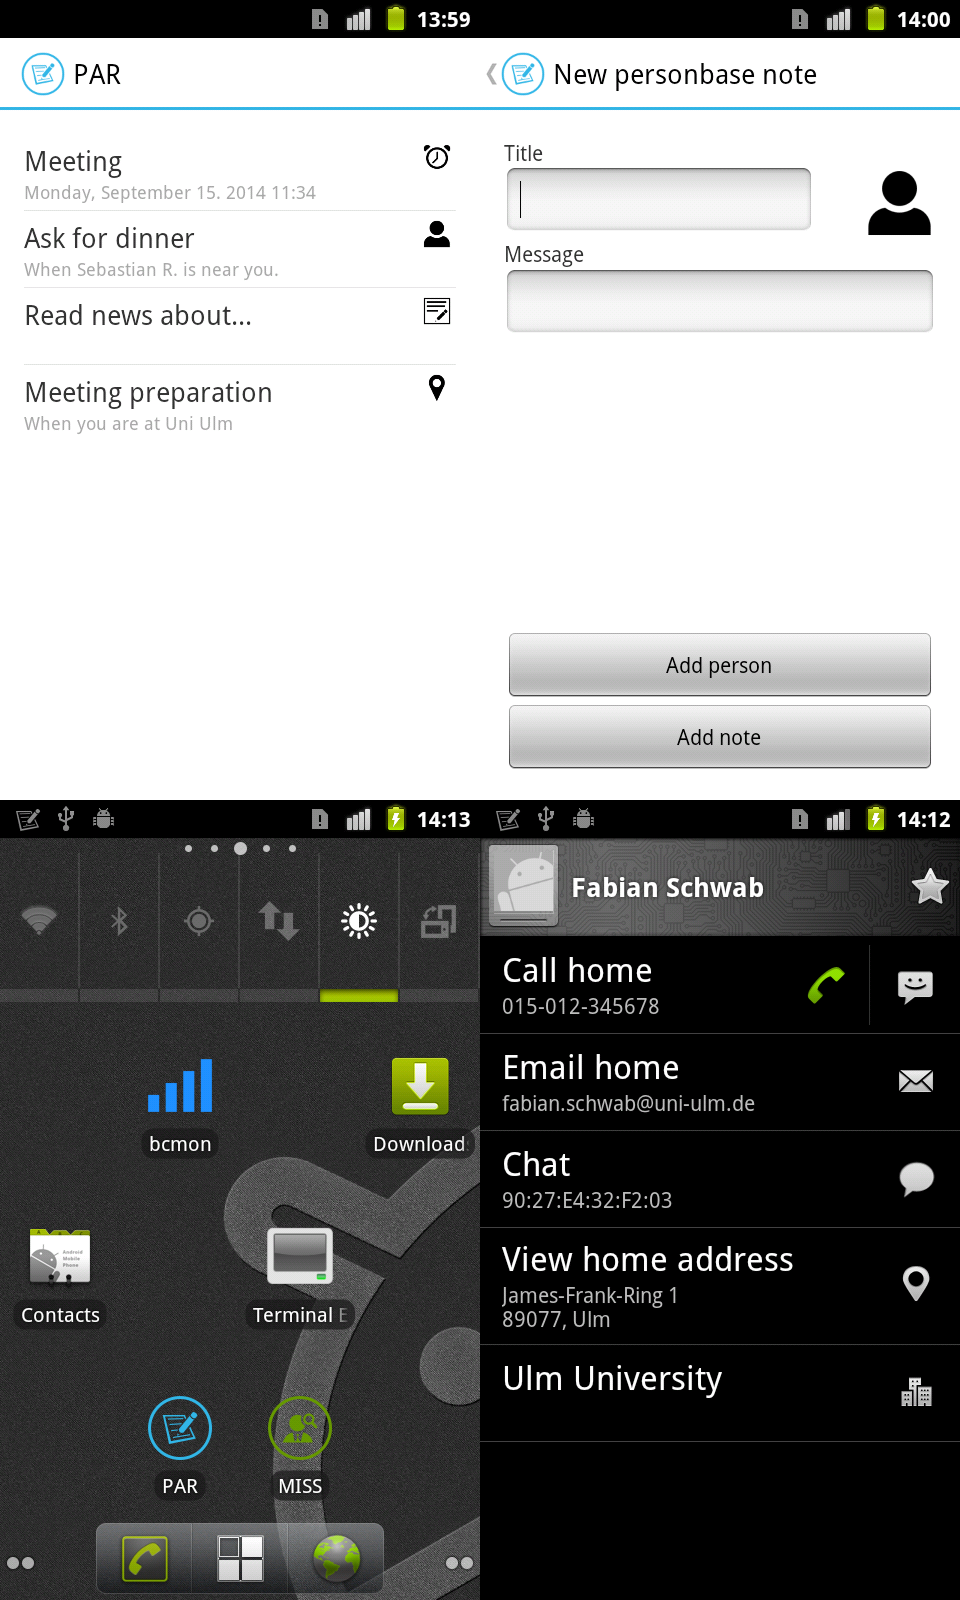
\includegraphics[width=4.0in]{bilder/par.png}
    \caption{Screenshots der Anwendung PAR und Notifikation in der Statusleiste.}
    \label{fig:par}
\end{figure}
\end{document}